\chapter{Implementation and Setup}\label{chap4}



\vspace*{40 ex}
%============================================================
\paragraph*{Outline:} This chapter presents the following:
\begin{enumerate}
\setlength{\itemsep}{-0.3em}
\item Introduction
\item Data Acquisition
\item Region Proposal Networks 
\item Edge Boxes Parameters
\item Faster R-CNN Architecture Model 
\end{enumerate}
%============================================================

\newpage

\section{Introduction}\label{chap4:intro}
In this chapter, we begin discussing the experimental part of the thesis. First, we will discuss selection criteria for models and datasets. Then we will describe the selected models, their parameters and the selected datasets. Finally, we will discuss postprocessing and evaluation. The implementation of the models is mostly discussed in the following chapter. However, some implementation details are also discussed in this chapter, since they influence method selection.


\section{Data Acquisition}
In this section, we will describe first, rice crop insect images dataset classification species and their labels  and next, rice crop weed images dataset.  

\subsection{Insects Data Exploration }

The dataset contains 814 images in which 723 training images and 91 test images, each of which belongs to one of fifteen species at several different growth stages(i.e Egg, Larva, Pupa and Adult.). We obtained the dataset through reference of  \href{http://www.knowledgebank.irri.org/step-by-step-production/growth/pests-and-diseases/insects}{Rice Knowledge Bank}, but originally the dataset has been taken from different sites and google search by the reference of this mention link and we have taken raw images of rice crop insects for their Complete Metamorphosis(Holometalolous) type according to their 4 stages and they are Egg, Larva, Pupa and Adult. The training images include the label of insect species, while the test images also include labels. We have used only the 723 training images to train a model and test the model accuracy.  

The input images are all square, but they have a wide range of pixel widths and heights, with some less than 100x100 pixels and some over 1000x1000 pixels, and each image has RGB colors. The figure 4.1 shows the distribution of pixel widths (also equal to the height distribution) for all input images. 



\begin{figure}
	\centering
	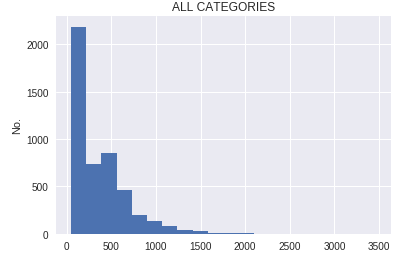
\includegraphics[width=0.7\linewidth]{img8}
	\caption{Histogram of insects dataset}
	\label{fig:img8}
\end{figure}


 I will need to rescale the input images to a uniform size to input into my neural network. A smaller uniform size makes the most sense, considering that many images are ~100 pixels on a side, and it’s easier to reduce the sizes of images than to reliably scale up the smaller images to a larger size. Also, using a smaller uniform size will help to save computational power. Therefore, I chose to rescale all images to the minimum size of the input data, 800 $\times$ 600.
 
 The input images include rice crop insects species from the following: Armyworms, Brown Plant Leafhopper , Gall Midge, Grasshopper, Leaf Folder, Mealy Bug, Paddy Stemborer, Rice Case Worm, Rice Earhead Bug, Rice Horned Caterpillar, Rice Skipper, Spiny Beetle, Thrips, White Backed Plant Hopper, Whorl Maggot. The table shown in the figure 4.2 gives the total number of each species, which range from 32 - 85
 
 \renewcommand{\arraystretch}{1.5}
 \begin{figure}[!ht]
	\centering
	\begin{tabular}{|c|c|c|c|c|}
		\hline
		Label& Species Class & Size & Totel\\ \hline
		1&Armyworms& 800 $\times$ 600 & 65 \\  \hline
		2 &Brown Plant Leafhopper & 800 $\times$ 600& 73\\  \hline
		3 &Gall Midge & 800 $\times$ 600& 32 \\  \hline
		4 &Grasshopper & 800 $\times$ 600& 74 \\  \hline
		5 &Leaf Folder & 800 $\times$ 600& 45\\  \hline
		6 &Mealy Bug & 800 $\times$ 600& 68\\ \hline
		7 &Paddy Stemborer& 800 $\times$ 600& 43 \\ \hline
		8 & Rice Case Worm & 800 $\times$ 600& 44\\ \hline
		9 &Rice Earhead Bug & 800 $\times$ 600& 48\\ \hline
		10 &Rice Horned Caterpillar & 800 $\times$ 600& 63\\ \hline
		11 &Rice Skipper & 800 $\times$ 600& 42\\ \hline
		12 &Spiny Beetle & 800 $\times$ 600& 85\\ \hline
		13 & Thrips & 800 $\times$ 600& 61\\ \hline
		14 & White Backed Plant Hopper & 800 $\times$ 600& 37\\ \hline
		15 & Whorl Maggot & 800 $\times$ 600& 36\\ \hline
		
	\end{tabular}
	
	\caption{Rice crop insects species list}
	\label{fig:img9}
\end{figure}

I split the 814 images into two different datasets: training set ( 88\%) and a test set (12\%). The training set is used to train the model and the test set is used to adjust weight parameters to check the loss function after training the model. Finally, the test set and other image serves to check the model accuracy using our scoring metrics and accuracy score. The images below are examples of each insect species of the input images. 
\noindent
\begin{figure}
	\centering
	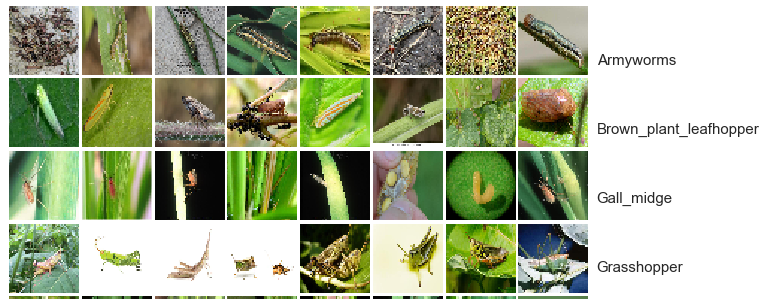
\includegraphics[width=\linewidth]{img10}
	\caption{Insects species name-I}
	\label{fig:img10}
\end{figure}
\noindent
\begin{figure}
	\centering
	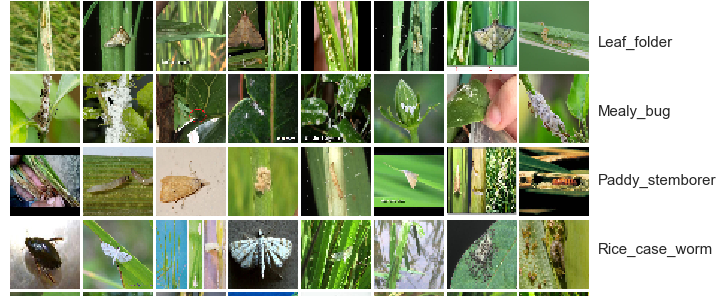
\includegraphics[width=\linewidth]{img11}
	\caption{Insects species name-II}
	\label{fig:img11}
\end{figure}
\noindent
\begin{figure}
	\centering
	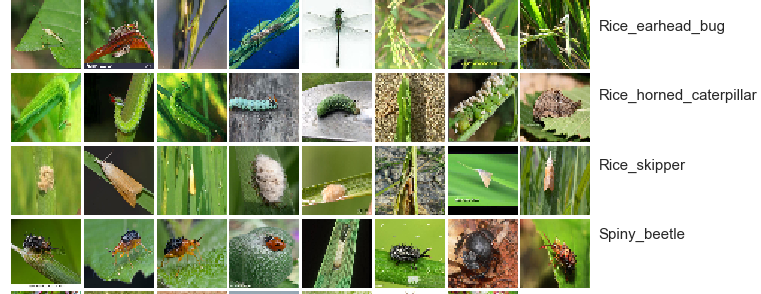
\includegraphics[width=\linewidth]{img12}
	\caption{Insects species name-III}
	\label{fig:img12}
\end{figure}
\noindent
\begin{figure}
	\centering
	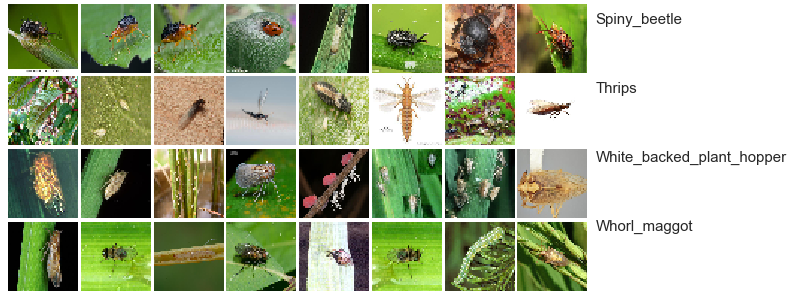
\includegraphics[width=\linewidth]{img13}
	\caption{Insects species name-IV}
	\label{fig:img13}
\end{figure}


\subsection{Weed Data Exploration }
The dataset contains 224 images in which 194 training images and 30 test images, each of which belongs to one of different growth stages of rice crop weed. We obtained the dataset through following dataset link \href{https://figshare.com/articles/rice_seedlings_and_weeds/7488830}{weed dataset},  but originally the dataset has been taken from the Figshare website. The training images include the label of weed species, while the test images also include labels. We have used only the 194 training images to train a model and test the model accuracy.



I will need to rescale the input images to a uniform size to input into my neural network. A smaller uniform size makes the most sense, considering that many images are ~100 pixels on a side, and it’s easier to reduce the sizes of images than to reliably scale up the smaller images to a larger size. Also, using a smaller uniform size will help to save computational power. Therefore, I chose to rescale all images to the minimum size of the input data, 800 $\times$ 600.

\section{Region Proposal Networks}

A Region Proposal Network (RPN) takes an image (of any size) as input and outputs a set of rectangular object proposals, each with an objectness score. We model this process with a fully convolutional network, which we describe in this section. Because our ultimate goal is to share computation with a Fast R-CNN object detection network, we assume that both nets share a
common set of conv layers. In our experiments, we investigate the Zeiler and Fergus model(ZF), which has 5 shareable conv layers and the Simonyan and Zisserman model (VGG), which
has 13 shareable conv layers.

To generate region proposals, we slide a small network over the conv feature map output by the last shared conv layer. This network is fully connected to an n $\times$ n spatial window of the input conv feature map. Each sliding window is mapped to a lower-dimensional vector (256-d for ZF and 512-d for VGG). This vector is fed into two sibling fully-connected layers—a box-regression layer (reg) and a box-classification layer (cls). We use n = 3 in this paper, noting that the effective receptive field on the input image is large (171 and 228 pixels for ZF and VGG, respectively). This mininetwork is illustrated at a single position in Figure 4.7. Note that because the mini-network operates in a sliding-window fashion, the fully-connected layers are shared across all spatial locations. This architecture is naturally implemented with an n $\times$ n conv layer followed by two sibling 1 $\times$ 1 conv layers (for reg and cls, respectively). ReLUs are applied to the output of the n $\times$ n conv layer. 
\noindent
\begin{figure}
	\centering
	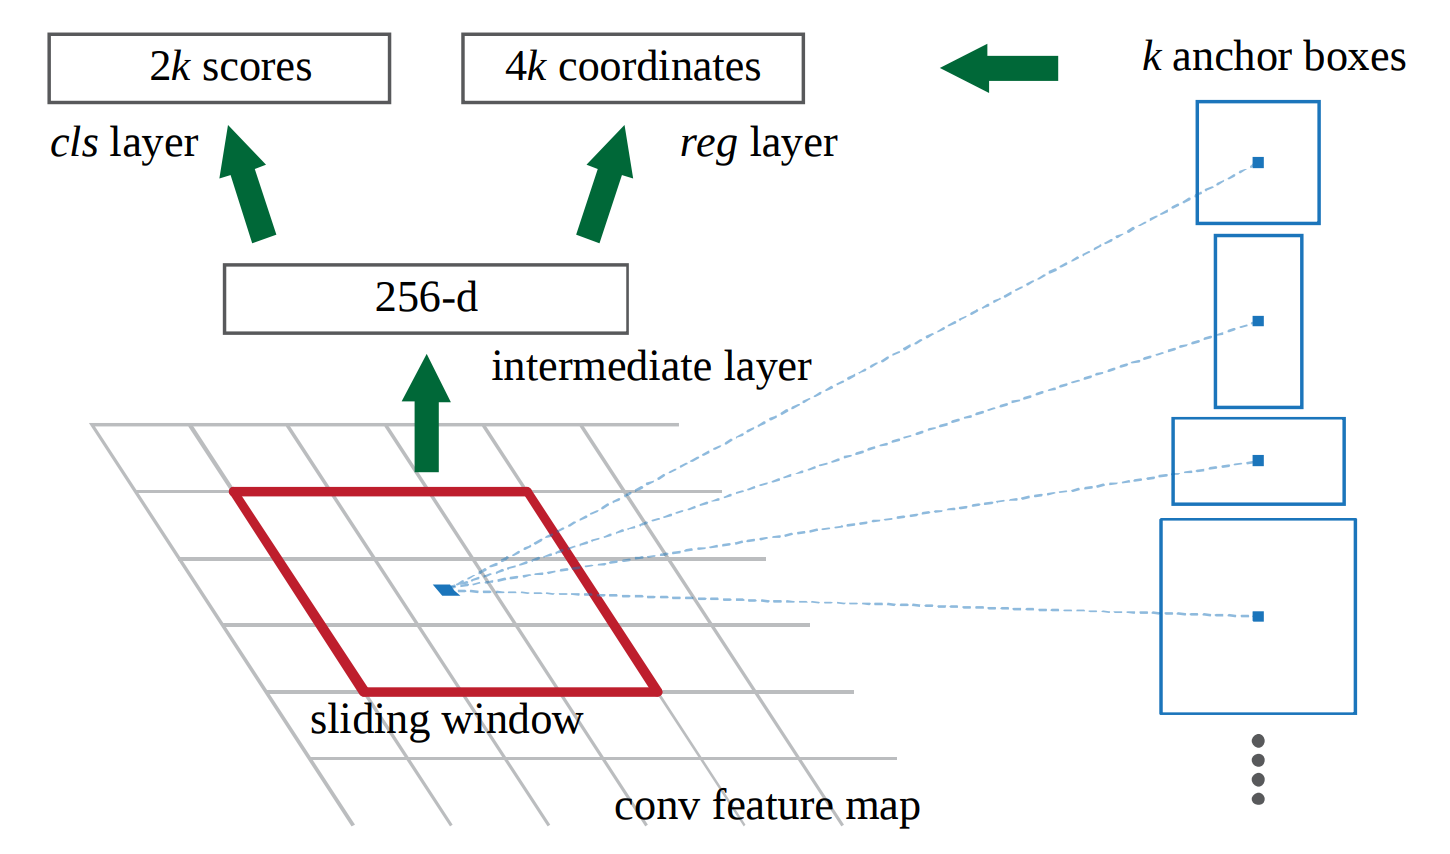
\includegraphics[width=\linewidth]{img16}
	\caption{Region Proposal Network (RPN)} \href{https://medium.com/@tanaykarmarkar/region-proposal-network-rpn-backbone-of-faster-r-cnn-4a744a38d7f9}{link}
	\label{fig:img16}
\end{figure}

\subsection{Translation-Invariant Anchors}

At each sliding-window location, we simultaneously predict k region proposals, so the reg layer
has 4k outputs encoding the coordinates of k boxes. The cls layer outputs 2k scores that estimate
probability of object / not-object for each proposal.2 The k proposals are parameterized relative to
k reference boxes, called anchors. Each anchor is centered at the sliding window in question, and is
associated with a scale and aspect ratio. We use 3 scales and 3 aspect ratios, yielding k = 9 anchors
at each sliding position. For a conv feature map of a size W $\times$ H (typically ~2,400), there are W Hk
anchors in total. An important property of our approach is that it is translation invariant, both in
terms of the anchors and the functions that compute proposals relative to the anchors.


As a comparison, the MultiBox method uses k-means to generate 800 anchors, which are not
translation invariant. If one translates an object in an image, the proposal should translate and the
same function should be able to predict the proposal in either location. Moreover, because the
MultiBox anchors are not translation invariant, it requires a (4+1) $\times$800-dimensional output layer,
whereas our method requires a (4+2) $\times$9-dimensional output layer. Our proposal layers have an order
of magnitude fewer parameters (27 million for MultiBox using GoogLeNet vs. 2.4 million for
RPN using VGG-16), and thus have less risk of overfitting on small datasets, like PASCAL VOC.

\subsection{A Loss Function for Learning Region Proposals}
For training RPNs, we assign a binary class label (of being an object or not) to each anchor. We
assign a positive label to two kinds of anchors: (i) the anchor/anchors with the highest Intersectionover-Union (IoU) overlap with a ground-truth box, or (ii) an anchor that has an IoU overlap higher
than 0.7 with any ground-truth box. Note that a single ground-truth box may assign positive labels
to multiple anchors. We assign a negative label to a non-positive anchor if its IoU ratio is lower than
0.3 for all ground-truth boxes. Anchors that are neither positive nor negative do not contribute to the
training objective.

With these definitions, we minimize an objective function following the multi-task loss in Fast RCNN. Our loss function for an image is defined as:\[L({p_{i}},{t_{i}}) = \frac{1}{N_{cls}} \sum_{i} L_{cls}(p_{i},p_{i}^{*}) + \lambda \frac{1}{N_{reg}} \sum_{i}p_{i}^{*} L_{reg}(t_{i},t_{i}^{*}) \]
\noindent
(Note : For simplicity we implement the cls layer as a two-class softmax layer. Alternatively, one may use logistic regression to produce k scores.)


Here, i is the index of an anchor in a mini-batch and $p_{i}$ is the predicted probability of anchor i being an object. The ground-truth label $p_{i}^{*}$ is 1 if the anchor is positive, and is 0 if the anchor is negative. $t_{i}$ is a vector representing the 4 parameterized coordinates of the predicted bounding box, and $t_{i}^{*}$ is that of the ground-truth box associated with a positive anchor. The classification loss $L_{cls}$ is log loss over two classes (object vs. not object). For the regression loss, we use $L_{reg} (t_{i} , t_{i}^{*}) = R(t_{i} - t_{i}^{*})$ where R is the robust loss function (smooth L1) defined in paper. The term $p_{i}^{*} L_{reg}$ means the regression loss is activated only for positive anchors $(p_{i}^{*} = 1)$ and is disabled otherwise $(p_{i}^{*} = 0)$. The outputs of the cls and reg layers consist of {$p_{i}$} and {$t_{i}$} respectively. The two terms are normalized with $N_{cls}$ and $N_{reg}$ , and a balancing weight $\lambda$.

For regression, we adopt the parameterizations of the 4 coordinates following :
\[t_{x} = (x - x_{a}) / w_{a}, t_{y} = (y - y_{a}) / h_{a} , t_{w} = log(w / w_{a}) , t_{h} = log(h / h_{a})\]
\[t_{x}^{*} = (x^{*} - x_{a}) / w_{a}, t_{y}^{*} = (y^{*} - y_{a}) / h_{a} , t_{w}^{*} = log(w^{*} / w_{a}) , t_{h}^{*} = log(h^{*} / h_{a})\]


where x, y, w, and h denote the two coordinates of the box center, width, and height. Variables x, $x_{a}$, and $x^{*}$are for the predicted box, anchor box, and ground-truth box respectively (likewise for y, w, h). This can be thought of as bounding-box regression from an anchor box to a nearby ground-truth box.

Nevertheless, our method achieves bounding-box regression by a different manner from previous
feature-map-based methods. In bounding-box regression is performed on features
pooled from arbitrarily sized regions, and the regression weights are shared by all region sizes. In
our formulation, the features used for regression are of the same spatial size (n $\times$ n) on the feature
maps. To account for varying sizes, a set of k bounding-box regressors are learned. Each regressor
is responsible for one scale and one aspect ratio, and the k regressors do not share weights. As such,
it is still possible to predict boxes of various sizes even though the features are of a fixed size/scale.

\subsection{Optimization}
The RPN, which is naturally implemented as a fully-convolutional network, can be trained
end-to-end by back-propagation and stochastic gradient descent (SGD). We follow the “imagecentric” sampling strategy from to train this network. Each mini-batch arises from a single image
that contains many positive and negative anchors. It is possible to optimize for the loss functions of
all anchors, but this will bias towards negative samples as they are dominate. Instead, we randomly
sample 256 anchors in an image to compute the loss function of a mini-batch, where the sampled
positive and negative anchors have a ratio of up to 1:1. If there are fewer than 128 positive samples
in an image, we pad the mini-batch with negative ones.

We randomly initialize all new layers by drawing weights from a zero-mean Gaussian distribution with standard deviation 0.01. All other layers (i.e., the shared conv layers) are initialized by pretraining a model for ImageNet classification, as is standard practice. We tune all layers of the ZF net, and conv3 1 and up for the VGG net to conserve memory. We use a learning rate of 0.001 for 60k mini-batches, and 0.0001 for the next 20k mini-batches on the PASCAL dataset. We also use a momentum of 0.9 and a weight decay of 0.0005. Our implementation uses Caffe.

\subsection{Sharing Convolutional Features for Region Proposal and Object Detection}
Thus far we have described how to train a network for region proposal generation, without considering the region-based object detection CNN that will utilize these proposals. For the detection network, we adopt Fast R-CNN and now describe an algorithm that learns conv layers that are shared between the RPN and Fast R-CNN.

Both RPN and Fast R-CNN, trained independently, will modify their conv layers in different ways.
We therefore need to develop a technique that allows for sharing conv layers between the two networks, rather than learning two separate networks. Note that this is not as easy as simply defining a single network that includes both RPN and Fast R-CNN, and then optimizing it jointly with backpropagation. The reason is that Fast R-CNN training depends on fixed object proposals and it is
not clear a priori if learning Fast R-CNN while simultaneously changing the proposal mechanism will converge. While this joint optimizing is an interesting question for future work, we develop a pragmatic 4-step training algorithm to learn shared features via alternating optimization.

In the first step, we train the RPN as described above. This network is initialized with an ImageNet-pre-trained model and fine-tuned end-to-end for the region proposal task. In the second step, we train a separate detection network by Fast R-CNN using the proposals generated by the step-1 RPN. This detection network is also initialized by the ImageNet-pre-trained model. At this point the two networks do not share conv layers. In the third step, we use the detector network to initialize RPN training, but we fix the shared conv layers and only fine-tune the layers unique to RPN. Now the two networks share conv layers. Finally, keeping the shared conv layers fixed, we fine-tune the fc layers of the Fast R-CNN. As such, both networks share the same conv layers and form a unified network.


\section{Edge Boxes Parameters}
As explained in section 3.3.3, Edge Boxes finds the initial region candidates using a sliding window search. The step size of the search is controlled by parameter $\alpha$, which defines the intersection over union (IoU) of neighbouring boxes. The same parameter defines the step size for translation, scale and aspect ratio. After the boxes have been found and refined, they are sorted and non-maximum suppression (NMS) is performed. During NMS, boxes are discarded if their IoU with a higher-ranking box is more than $\beta$.

$\alpha$ and $\beta$ are the most important parameters of Edge Boxes. The authors of the method studied the effect of these parameters from the perspective of finding a suitable candidate accuracy for the object detector. Even though an IoU value higher than 0.5 is typically used as the criterion for evaluating the performance of an object detector (as the limit for determining true matches), the object detector often performs better, if the candidate objects are a closer match to true objects. Thus, the target IoU should be set higher than the minimum acceptable IoU. 

The authors define the target IoU as $\delta$ and performed experiments with $\delta$ values of 0.5, 0.7 and 0.9. Since Fast R-CNN in any case calculates refinements of the bounding boxes, we decided that increasing $\delta$ above 0.9 is not needed for the present experiments. The resulting increase in the number of candidates would only slow down the algorithm. We chose a more practical value $\delta$ = 0.7 as the target IoU. 

$\alpha$ and $\beta$ are set according to $\delta$. If a higher value of $\delta$ is required, $\alpha$ and $\beta$ are selected to output denser sets of bounding boxes around apparent objects. The authors found that a value of $\alpha$ = 0.65 provided the best results for $\delta$ $<$ 0.9. The optimal value of $\beta$ was determined to be $\delta$ $+$ 0.05. Thus, we chose $\alpha$ = 0.65 and $\beta$ = 0.75 as the parameter values. 

For the minimum objectness score limit $h^{in}_{b}$ (used for discarding uninteresting windows before the refinement stage), we used the default value of 0.01. We also used the default value of 10,000 as the maximum number of object proposals.

\section{Faster R-CNN Architecture Model}

One of the state-of-the-art object detection models is Faster R-CNN. The architecture of Faster R-CNN is shown in Figure 4.8. Given an image, we first employ a pre-trained deep convolutional neural network, such as VGG, to extract feature maps from it. Then, they use a Region Proposal Network (RPN), which consists of two convolutional layers, to detect the regions that might contain object in the feature maps (image). Then the network employ a RoI pooling layer to crop and resize the the feature maps according to these region proposals. The new feature maps of each region are then used for classification and finer bounding box regression through three fully connected layers.

\begin{figure}
	\centering
	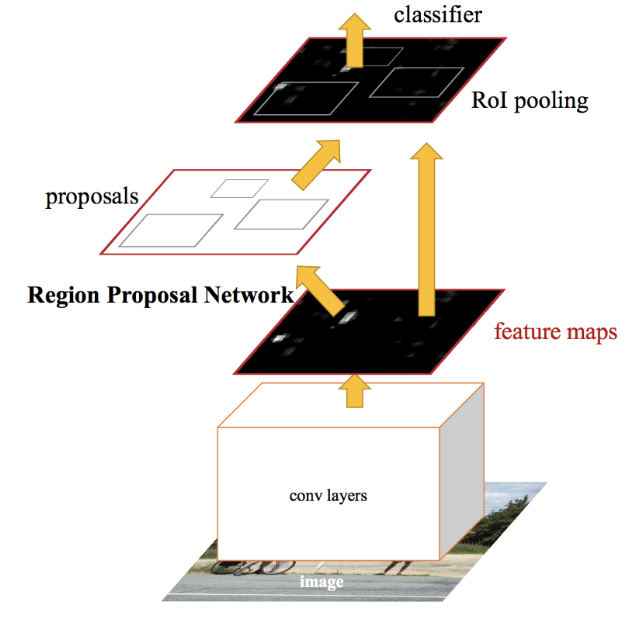
\includegraphics[width=\linewidth]{img7}
	\caption{Architecture of Faster R-CNN} \href{https://medium.com/@tanaykarmarkar/region-proposal-network-rpn-backbone-of-faster-r-cnn-4a744a38d7f9}{link}
	\label{fig:img7}
\end{figure}

One issue of this Faster R-CNN architecture is that the region proposals output from RPN are not very accurate. This is due to RPN using some hard coded anchors with fixed scales and aspects to guess the potential regions. Although RPN also has a bounding box regression part, it only aims to give general boxes that may contain any kind of objects. Without class specific knowledge, these boxes won’t be very accurate. We argue that the error of classification and final bounding box regression might be partly caused by error of proposed region. Suppose we can have finer region proposals, the accuracy of classification and final bounding box regression may be further improved.

\subsection{Iterative Region Proposal Refinement Model}
A nature better region proposal will be the regressed bounding box since it is designed to refine the rough region output by RPN using class specific knowledge encoded in the network. Since regressed bounding box is one of the outputs of the whole Faster R-CNN network, we cannot use it as our region proposal at the beginning. However, once we get the finer bounding box, we can start another round of classification and bounding box regression, using the regressed bounding box in previous round as the region proposals in the new round. This process can keep going for several iterations. In this iterative way, we can refine the region proposals again and again and might get a better result after each iteration.

The model of Faster R-CNN with iterative region proposal refinement is shown in Figure 4.9. In the first iteration, it’s exactly the same as Faster R-CNN: extract feature maps from image by VGG, pass them to RPN to get region proposals, employ RoI pooling layer to crop and resize new feature maps for each proposal, and use a three-layer fully connected network to get the final class scores and bounding box regression for each class.

After the first iteration, for each proposed region, we select the regressed bounding box with the maximum class score as the region proposal in the second iteration. And the rest of second iteration is the same as the first iteration: we use RoI pooling layer to crop and resize feature maps for each proposal, classify and regress the bounding box using new feature maps. Note that for the input of RoI pooling layer, we reuse the feature maps in first iteration and there is no need for recalculation. Also, we reuse parameters of the three-layer fully connected network in different iterations. After the second iteration, we can repeat the same process for the third iteration, and so on. Figure 4.9 is a demonstration of iteration number = 3.

Our iterative refinement model can be represented by the following equations. For the feature maps extraction and each initial RPN region proposal, we have
\[f = VGG(image)\]
\[RP_{1} = RPN(f)\]

Then suppose we set iteration number = T, then for each iteration i, the model can be represented as : 

for i =1, 2, ...T,

\[  r_{i} = RoIPooling(f,RP_{i})\]
\[scores_{i} , boxes_{i} = FC^{3}(r_{i}) \]
\[RP_{i+1} = boxes_{i , arg  max_{j \in 0... C}scores_{ij}} \]
\[loss_{i} = loss_{cross-entropy}(scores_{i} , C_{i}) + \lambda [c \neq bg ] loss_{smooth_{L1}} (boxes_{i} , b_{i})\]

where $FC^{3}$ denotes the three-layer fully connected network, C denotes the number of classes, $c_{i}$ denotes the class
label for the proposed region $RP_{i}$ , $b_{i}$ denotes the ground truth bounding box of object in this region,[$c_{i} \neq b_{g}$] = 1 if the region is not a background and contains object, otherwise [$c_{i} \neq b_{g}$] = 0, and $\lambda$ is the weight parameter to balance classification loss and bounding box regression loss.

During training, for the classification, we use softmaxcross entropy loss, and for the bounding box regression, we use smooth L1 norm loss. We will get a $loss_{i}$ in each iteration. The final loss will be the sum of all iterations (loss from RPN might also be added to the final loss). And in test time, we use the scores and bounding boxes from the last iteration as the final output:
\[loss_{final} = \sum_{i=1}^{T} loss_{i}\]
\[output = scores_{T} , boxes_{T}\]
\begin{figure}
	\centering
	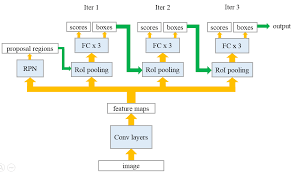
\includegraphics[width=\linewidth]{img18}
	\caption{Architecture of Faster R-CNN with iterative region proposal refinement} \href{http://cs231n.stanford.edu/reports/2017/pdfs/112.pdf}{link}
	\label{fig:img18}
\end{figure}


\subsection{LSTM Region Proposal Refinement Model}
One issue of the iterative refinement model is the gradient of loss can not be backpropagated from the later iteration to the earlier iterations. Since the error of classification and bounding box regression of later iteration might be
caused by errors of earlier iterations, we hope those earlier
errors can also be corrected by gradient backpropagation.
However, this cannot be done by iterative refinement model
since RoI layer cannot backpropagate the gradient to the region proposal coordinates. This is because RoI layer uses
these coordinates to crop the feature maps, but the ”crop”
operation is not differentiable with respect to coordinates.
As a result, in Figure 4.9 the gradient of each loss in iterative
model can only be propagated downward (yellow arrows) but cannot be propagated to the left (green arrows).

Inspired by Reccurrent Neural Network (RNN), which
can pass useful information to later time steps and also
propagate the gradient backward to the previous time steps,
we propose a LSTM region proposal refinement model,
where LSTM is one of RNN models. The architecture of
our model is shown in Figure 4.10. The different between iterative and LSTM refinement models is that we add a LSTM
layer right before the final fully connected (output) layer,
and pass the hidden states of LSTM to the next iteration
(blue arrows). As a result, if the iteration number = T, then
in each iteration i, the equations become

for i =1, 2, ...T

\[  r_{i} = RoIPooling(f,RoI_{i})\]
\[a_{i} = FC^{2} (r_{i})\]
\[h_{i} = LSTM(h_{i-1} , a_{i})\]
\[scores_{i} , boxes_{i} = FC(h_{i})\]
\[RoI_{i+1} = boxes_{i , arg  max_{j \in 0... C}scores_{ij}} \]
\[loss_{i} = loss_{cross-entropy}(scores_{i} , C_{i}) + \lambda [c \neq bg ] loss_{smooth_{L1}} (boxes_{i} , b_{i})\]


where $h_{i}$ is the hidden state of LSTM at iteration i, and the input of the LSTM layer is $h_{i}$ - 1, the hidden state of previous iteration, and $a_{i}$, the output of two-layer fully connected network in current iteration. The rest of this model is the same as iterative refinement model.

One benefit of adding a LSTM layer is that the hidden
state of previous iteration can contain information that is
useful to improve classification and bounding box regression results in current iteration. Another benefit is that we
can now backpropagate the gradient of loss from the later
iterations to the earlier ones (through the blue arrows in Figure 4.10), since LSTM is differentiable with respect to the previous hidden state. As a result, if the error of prediction
in current iteration comes from the errors of previous iterations, LSTM gives it a chance to correct those errors by
gradient backpropagation.


Actually, this is an unusual use of LSTM/RNN model.
RNNs are more often used in sequential input data such as
text, audio and video. The hidden state of RNN was proved
to have the ability to capture the temporal information of
data at previous time steps. Since the meaning of current
frame in sequential data is often related to the frames previous to it, RNN makes a great success in encoding features
of sequential data.


Although our data is image, which is not sequential
data, but the way we refine the region proposals and make
progress step by step also contains temporal information.
We can see the iterations as multiple guesses. In each iteration, we look into the guessed region of the image and get
some information that is useful to decide a better guess next time. This way of sequential processing of non-sequential
data is often called attention or glimpse model, which has
been used in both multiple object detection and question
answering . In the paper, they also use a LSTM to
refine the answer span for a question for multiple times.

\begin{figure}
	\centering
	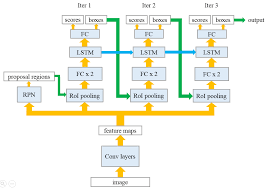
\includegraphics[width=\linewidth]{img19}
	\caption{Architecture of Faster R-CNN with LSTM region proposal refinement.} \href{http://cs231n.stanford.edu/reports/2017/pdfs/112.pdf}{link}
	\label{fig:img19}
	\end{figure}
%++++600+++++++++++++++++++++++++++++++++++++++++++++++++++++++++++++++++++++++++++++
%\section{Summary}
%\label{chap4:sum}
%In this chapter....

